% ·-·-·-·-·-·-·-·-·-·-· [格式部分] ·-·-·-·-·-·-·-·-·-·-·-· %
%!TEX program = xelatex
\documentclass[twocolumn]{article}
\setlength{\columnsep}{1.2cm}

\usepackage[UTF8]{ctex}
\usepackage{graphicx} %插入图片的宏包
\usepackage{float} %设置图片浮动位置的宏包
\usepackage{subfigure} %插入多图时用子图显示的宏包
\usepackage[colorlinks,linkcolor=blue,anchorcolor=blue,citecolor=green]{hyperref}
\usepackage{amsmath}
\usepackage{fontspec}
%文件中可以有超链接的宏包并且可以为其设定样式
\usepackage{float}
\usepackage{overpic}

\usepackage{authblk}

%edge
\usepackage{geometry}
\geometry{a4paper,left=1.2cm,right=1.2cm,top=1cm,bottom=1.5cm}
%color
\usepackage{color}
%\pagecolor[rgb]{0.1568,0.1607,0.1373}\color{white}%全同灰
%\pagecolor[rgb]{0,0,0}\color{white}%极致黑
\usepackage{listings}
\usepackage{xcolor}
\lstset{
framexleftmargin=1mm,
 frame=shadowbox, 
 rulesepcolor=\color{blue}}
% ·-·-·-·-·-·-·-·-·-·-· [概要部分] ·-·-·-·-·-·-·-·-·-·-· %
	\title{\bf NoGo不围棋大作业结题报告}
  \author{欧阳霄宇 \thanks{2000017709@stu.pku.edu.cn} \ 李傲骋 \thanks{2000017706@stu.pku.edu.cn}}


	\date{\today}
\begin{document}

\maketitle{}
\tableofcontents
\newpage
% ·-·-·-·-·-·-·-·-·-·-· [正文部分] ·-·-·-·-·-·-·-·-·-·-· %
\part{摘要}
本文介绍了两人合作开发的不围棋(NoGo)游戏程序开发过程与软件特点。软件主要包括游戏规则部分、AI部分与人机交互部分,两人分工合作共同完成了软件编写。我们的不围棋程序具有选择菜单、复盘、暂停存档、悔棋等多种功能,AI基于负极大值算法编写,满足作业基本要求。在此基础上,我们完善了人机交互功能,提供了不同的交互方式(键盘输入或鼠标交互)、不同算法的AI、不同对战模式(人机对战、人人对战、AI对战)等等。
\part{基本功能部分}
\section{气的计算}
无论是在不围棋或围棋中,棋子的“气”都是决定胜负的重要因素。因此棋盘上每个棋子的气在判断输赢或计算局面估值中都非常重要。在大部分常见裁判程序中,程序通过递归判断一片连接成块的棋子周围是否有未落子的点来判断棋子{\bf 是否}有“气”,而在我们的程序中,我们递归计算得出了气的{\bf 点数}:即,{\it 一个棋子的“气”(air)是与其连接在一起的所有同色棋子周围的未落子点个数之和。}例如,下面的图\ref{Fig.main}给出了一个棋盘样例和程序计算出的气的分布。
\begin{figure}[H]
\centering  %图片全局居中
\subfigure[棋盘样例]{
\label{Fig.sub.1}
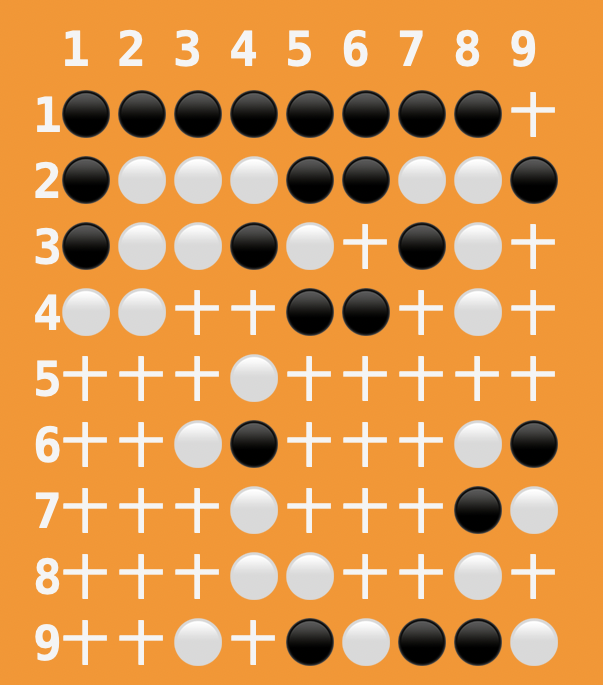
\includegraphics[width=0.2\textwidth]{fig1}}
\subfigure[气的分布]{
\label{Fig.sub.2}
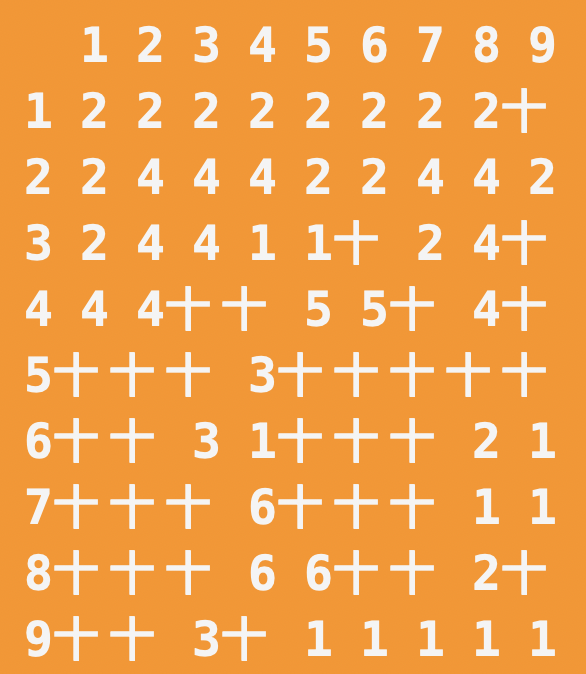
\includegraphics[width=0.2\textwidth]{fig2}}
\caption{气的分布示意}
\label{Fig.main}
\end{figure}
\par
在源代码中,我们的“multiAir”函数与“tag”函数用于计算每个点的气数。这两个函数在终局判断、估值函数的建立与调试、AI算法的不断改进中起了重要作用。
\section{终局判定}
按照不围棋规则,若对弈不允许空手,则游戏结束时,必然是最后落子的一方判负,最后负方落子被判负的点可以分为两种情况:
\par
一是下在这个点导致这个点棋子气为0,按照规则会被对方提走,这种下法在不围棋中是直接禁止的。这些点可简称为禁止点(在程序中称为Forbid Point):{\it 若对于黑棋来说,一个空点四周所有的点均为白棋、边界或只有一口气的黑棋,则这个点称为黑棋的禁止点。}
\par 
二是下在这个点导致周围对方的点的气变为0,按照不围棋规则,此时落子方因为提走了对方的棋子,落子方判负。这种点可称为死点(在程序中称为Dead Point):{\it 若对于黑棋来说,一个空点四周存在一个白子且白子的气为1,则这个点称为黑棋的死点。}

\begin{figure}[H]
\subfigure[黑棋的禁止点与死点]{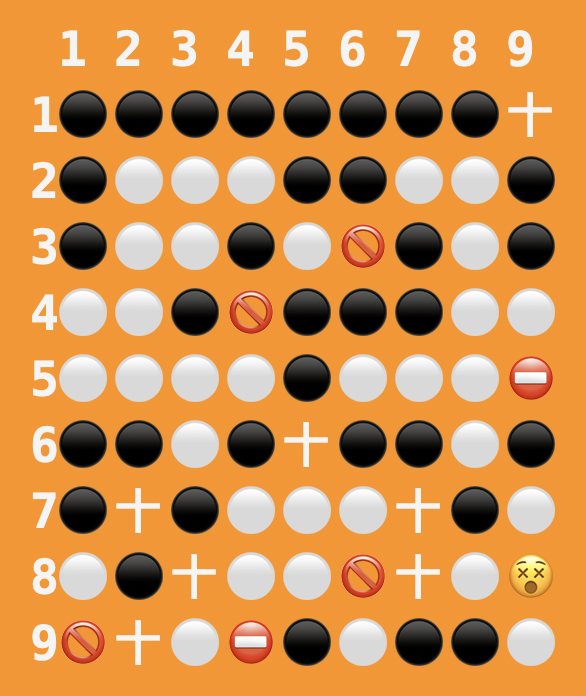
\includegraphics[height=4cm]{fig3}}
\subfigure[白棋的禁止点与死点]{
    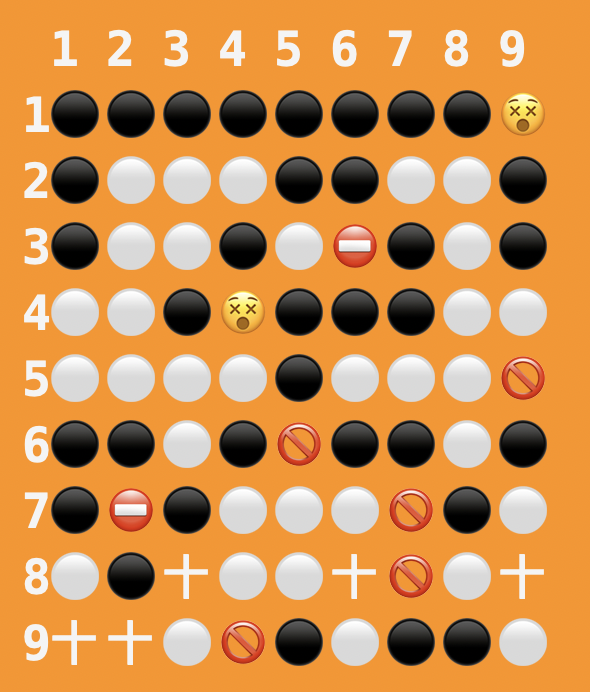
\includegraphics[height=4cm]{fig4}
}
\subfigure[符号]{
	\begin{minipage}[b]{0.1\linewidth}
    
\includegraphics[height=1.2cm]{emoji1.png}
    
\includegraphics[height=1.2cm]{emoji2.png}
    
\includegraphics[height=1.2cm]{emoji3.png}
    \end{minipage}
}
\caption{禁止点与死点的例子。图(c)的三个符号分别代表禁止点、死点和既是禁止点、也是死点的点。}
\end{figure}

\par
在程序中,禁止点用judgeForbidPoint函数判断,死点用judgeDeadPoint函数判断。一旦有一方的棋子落到了自己的禁止点和死点上,即立刻判负。


\part{机器算法部分}
\section{负极大值算法}
负极大值算法:
在棋局的每个状态,比如轮到A走棋了,那么我们会遍历A的每一个可能走棋方法,然后对于前面A的每一个走棋方法,遍历B的每一个走棋方法,然后接着遍历A的每一个走棋方法,如此下去,直到得到确定的结果或者达到了搜索深度的限制。当达到了搜索深度限制,此时无法判断结局如何,但通过气和眼对优劣势进行估值(value),选择使己方value
最大、对方value最小的落子位置。指定搜索层数,便可以进行博弈。

\begin{lstlisting}[language=C++]
step AI(int chess)//AI,负极大值算法
{
step result;
result.chess = chess;
int max = -1000;
for (int t1 = 0; t1 < 9; t1++) 
{
  for (int t2 = 0; t2 < 9; t2++) 
  {
   if (board[t1][t2] == 0 &&
   judgeForbidPoint(chess, t1, t2)==0 
   &&
   judgeDeadPoint(chess, t1, t2)==0) 	                                
   {		
      int tmp_value = 
         value(t1, t2, chess, 0);
      if (max < tmp_value)
      {
        max = tmp_value;
        result.x = t1;
	    result.y = t2;
      }
   }
  }
}
return result;
}
\end{lstlisting}


\section{MCTS算法}
MCTS算法需要建立蒙特卡洛树,在棋局每产生一种新状态时,AI先随机选择可以下的位置进行快速随机落子,并且在每个节点产生对局数和胜局数,然后继续向下搜索,在每一层选择一个胜率和对局数都高的位置进行落子,直到达到最深的节点,然后快速随机落子,判断出输赢后,在每个父节点加一个对局数和输赢状态。在进行大量选择、扩展、模拟、回溯后,选择第一层胜率和对局数都高的位置进行落子。
\begin{figure}[H]
\centering  %图片全局居中
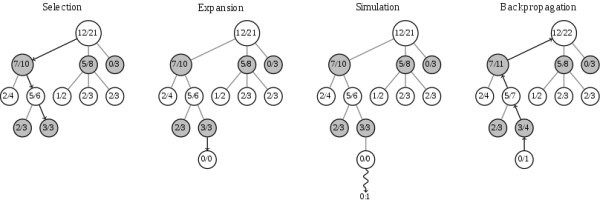
\includegraphics[width=0.5\textwidth]{fig51}
\caption{蒙特卡洛树}
\label{Fig.main}
\end{figure}

在综合判断胜率和对局数时需要用到UCT公式

$$score=x_{child}+C\cdot \sqrt{\frac{\log(N_{parent})}{N_{child}}}$$
其中$x_{child}$是节点的胜率,$N_{parent}$是该层所有对局数的和,$N_{child}$是该节点对局数,C作为参数衡量了对局数的重要性,因为一个节点对局数越多,越代表它比其他同级节点更容易被选中,也即更容易胜利。C在前后不同的阶段可以取不同的值。

\par

蒙特卡洛树的实现需要链表储存胜局数、对局数和父节点、子节点以进行选择、扩展、模拟、回溯。

\par

以下为代码部分截图,但由于略复杂,目前还未完成。
\begin{figure}[H]
\centering  %图片全局居中
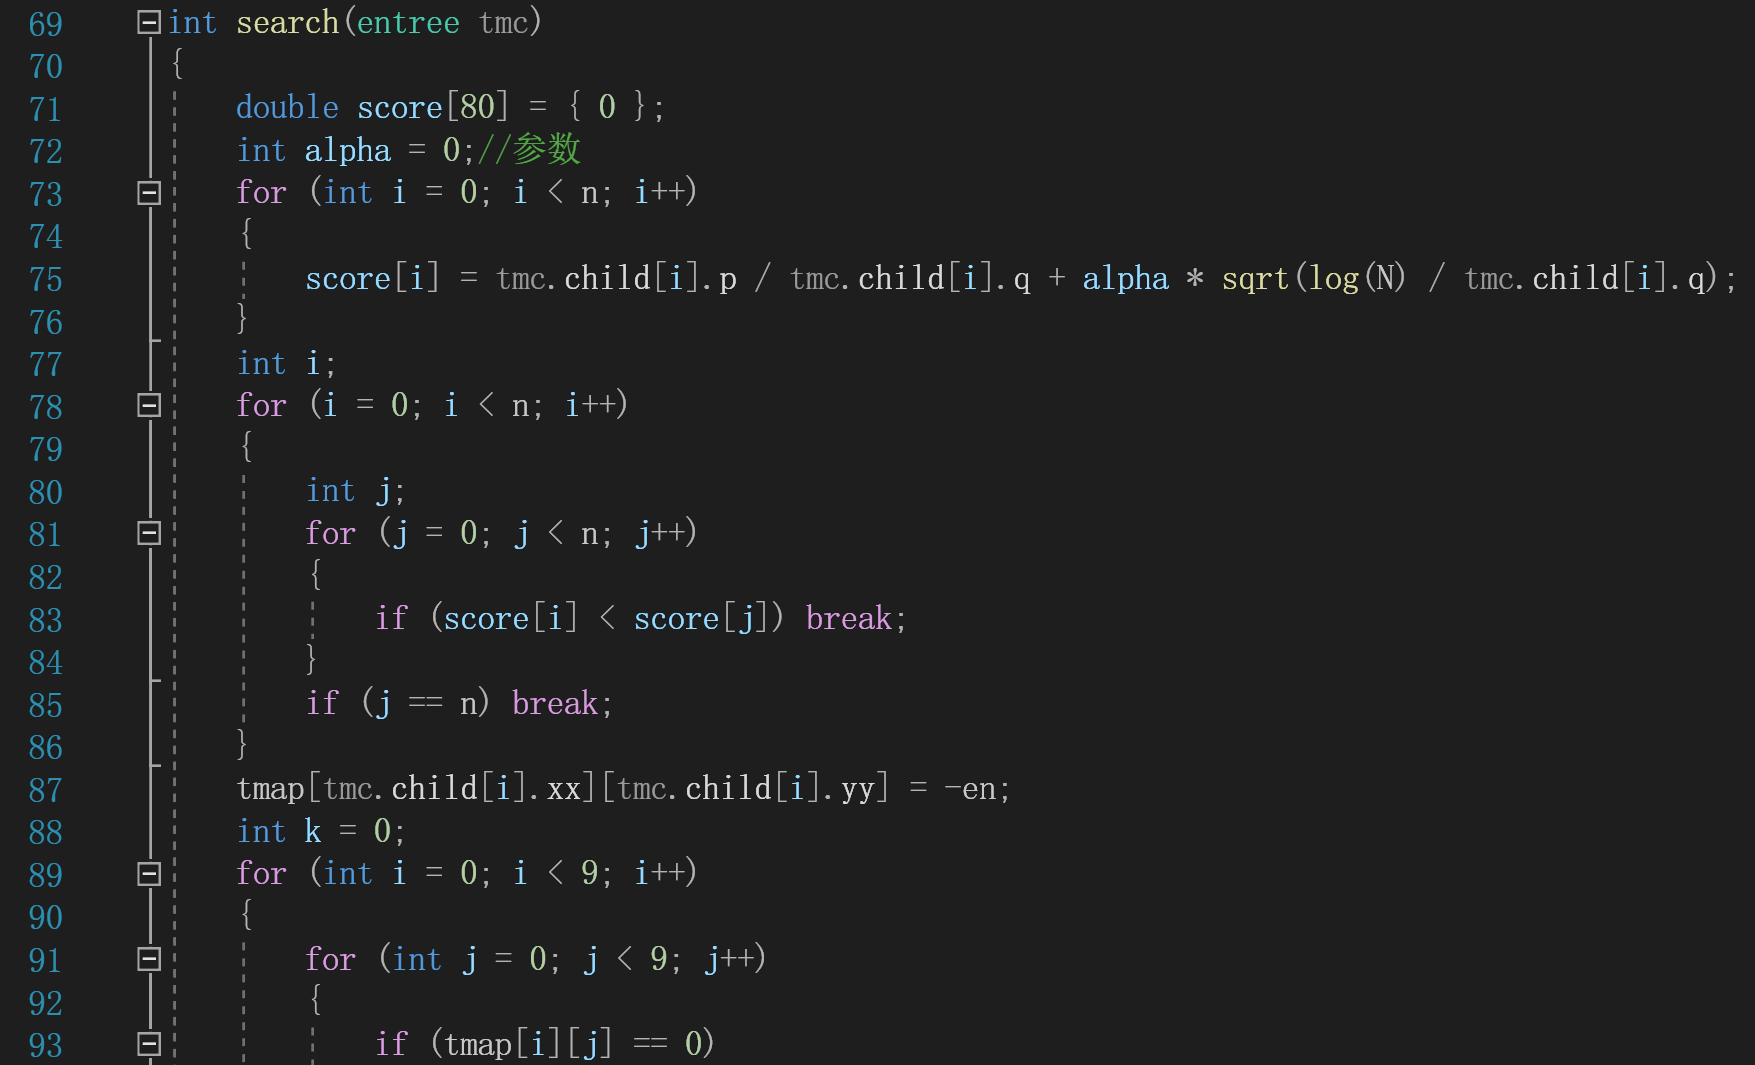
\includegraphics[width=0.5\textwidth]{fig81}
\caption{搜索函数}
\label{Fig.main}
\end{figure}

\begin{figure}[H]
\centering  %图片全局居中
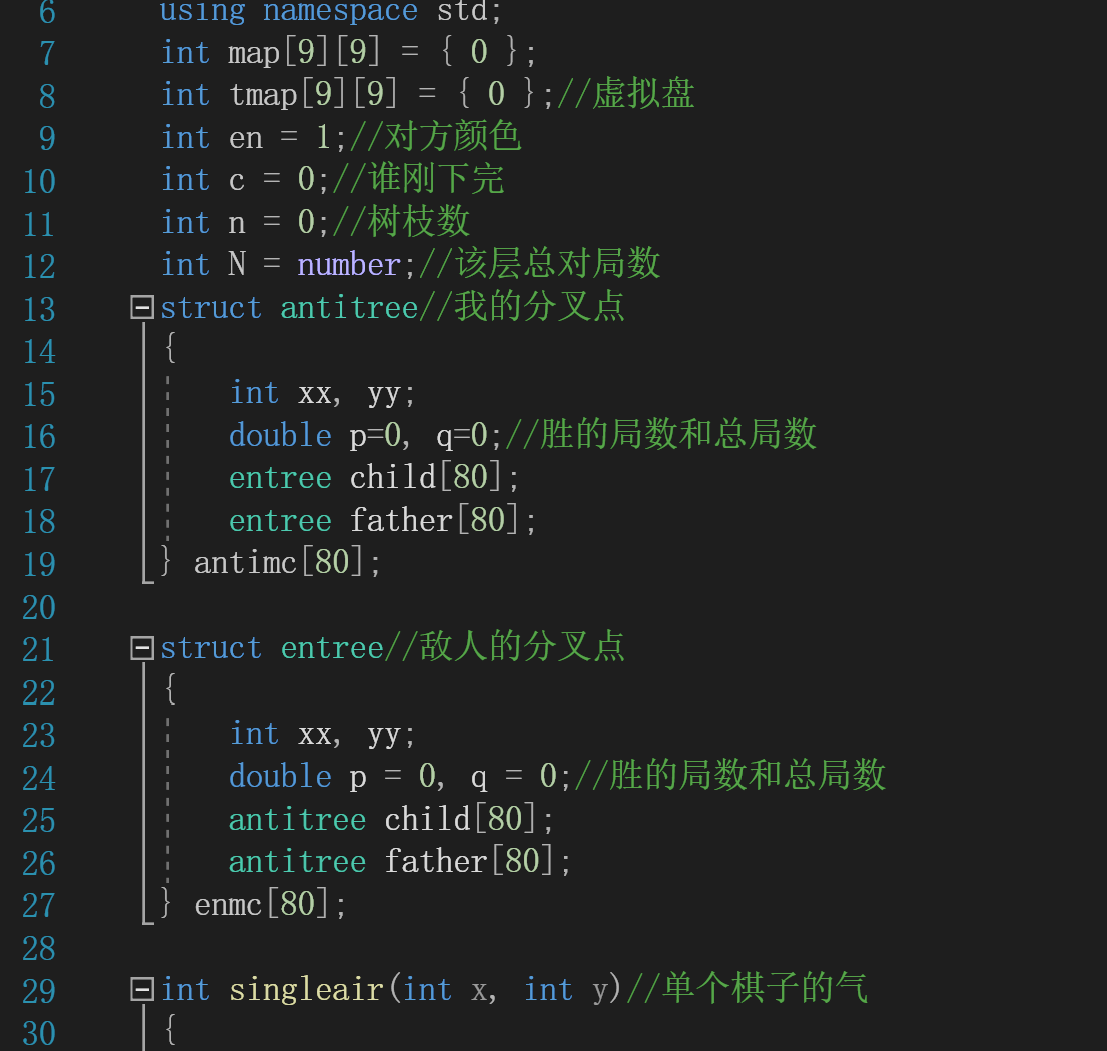
\includegraphics[width=0.4\textwidth]{fig71}
\caption{节点结构体}
\label{Fig.main}
\end{figure}

\section{实际程序算法特点}
实际程序中的AI基于负极大值方法编写。然而,由于搜索层数较大,在开局阶段,负极大值搜索方法速度较慢(统计约为1s左右),且开局估值差异较小,无需深层搜索。因此实际的程序采用了这样的解决方案:当轮数低时(轮数小于15时),通过完善一轮估值函数,仅进行一轮估值,得出结果(AI在程序中名为小黄鸭)。轮数较高时,深层负极大值搜索得出的结果质量更高,且计算时间在可接受范围内,故此时选用深层搜索AI(在游戏中名为大黄鸭)。
\par
“小黄鸭”估值函数的构成具有如下特点:
\begin{enumerate}
{\it
	\item {估值与棋子落在该点之后的气数负相关;}
	\item {估值与该点四周同样颜色的棋子的个数负相关;}
	\item {估值与该点四周可能形成“眼”的可能性正相关。}
}
\end{enumerate}
\par
“大黄鸭”估值函数的构成具有如下特点:
\begin{enumerate}
{\it
	\item 估值与局面上己方不能下的禁止点和死点个数负相关;
	\item 估值与局面上对方不能下的禁止点和死点个数正相关。
}
\end{enumerate}
\par 
然而由于开发中的种种问题,我们只使用了早期版本的大黄鸭AI参加botzone比赛。由于botzone平台上有着1s的超时限制,我们80\% 的棋局都以超时憾负。在最终的比赛中,我们的AI取得了2胜7(实际未超时局数3局,有效胜率2/3)的成绩,非常遗憾!我们痛定思痛、吸取教训,在调整了AI算法后,我们的AI发挥稳定,甚至还在botzone平台中击败了基于MCTS算法、排名前10的某bot(如图\ref{大黄鸭}所示),算是差强人意。
\begin{figure}[H]
\centering  %图片全局居中
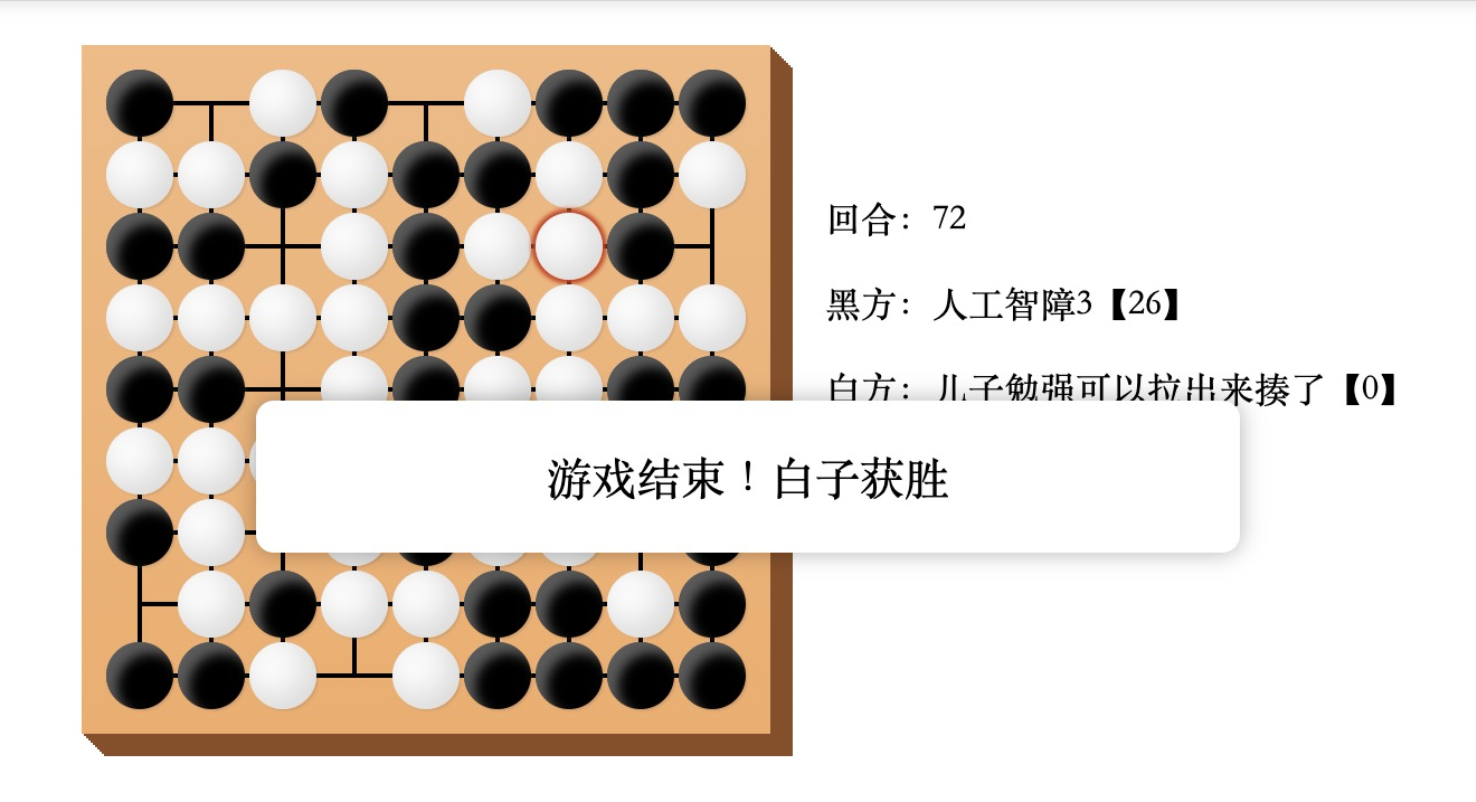
\includegraphics[width=0.4\textwidth]{fig15}
\caption{大黄鸭AI(白方)战绩喜人}
\label{大黄鸭}
\end{figure}

\part{交互界面部分}
\section{终端交互界面}
\subsection{基本模式}
较为基础、功能较全面的终端交互界面如图\ref{Fig3}所示。终端交互界面提供三种模式:人机对战模式、人人对战模式、观看AI对局模式。
\subsubsection{人机对战模式}
传统的人机对战模式支持先后手选择(即黑白棋选择)、支持自由选择难度由易至难的3个AI、支持对弈玩家悔棋(即AI先撤回上一步棋,玩家也撤回上一步棋)。
\begin{figure}[H]
\centering
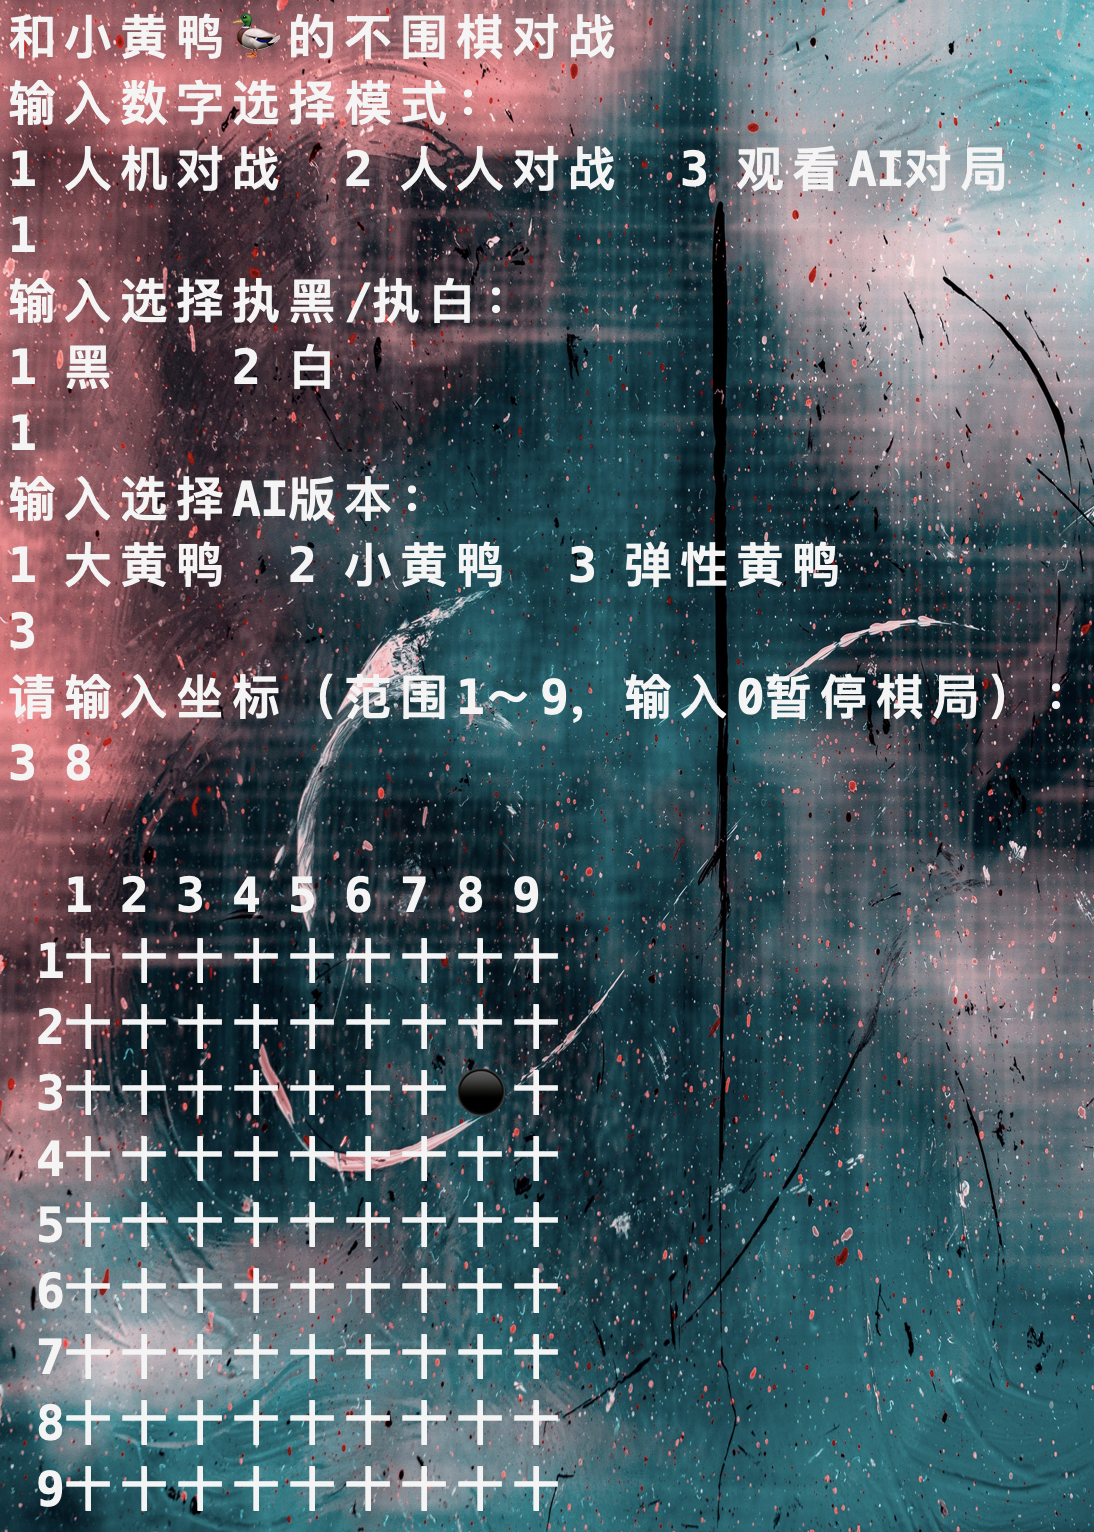
\includegraphics[width=0.3\textwidth]{fig5}
\caption{人机对战模式的终端交互界面}
\label{Fig3}
\end{figure}
\subsubsection{观看AI对战}
如图\ref{Fig4}所示,AI对局模式允许玩家自由在3个AI中选择,并指定黑棋和白棋各自的AI,观看两个AI之间对战。这种模式的特点是玩家可以在观看AI对弈中了解每个AI的特点、强弱,便于调试;且AI本身运行速度快,玩家在观看中,可以短时间内掌握游戏技巧、理解游戏规则。
\begin{figure}[H]
\centering
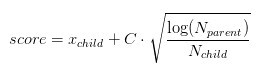
\includegraphics[width=0.3\textwidth]{fig6}
\caption{观看AI对战的终端程序界面}
\label{Fig4}
\end{figure}
\subsubsection{人人对战模式}
为了方便玩家两两之间的切磋,程序还加入了对于人人对战的支持。玩家在终端界面通过键盘输入棋盘坐标落子,黑白两者交替落子,如图\ref{Fig5}所示。
\begin{figure}[H]
\centering
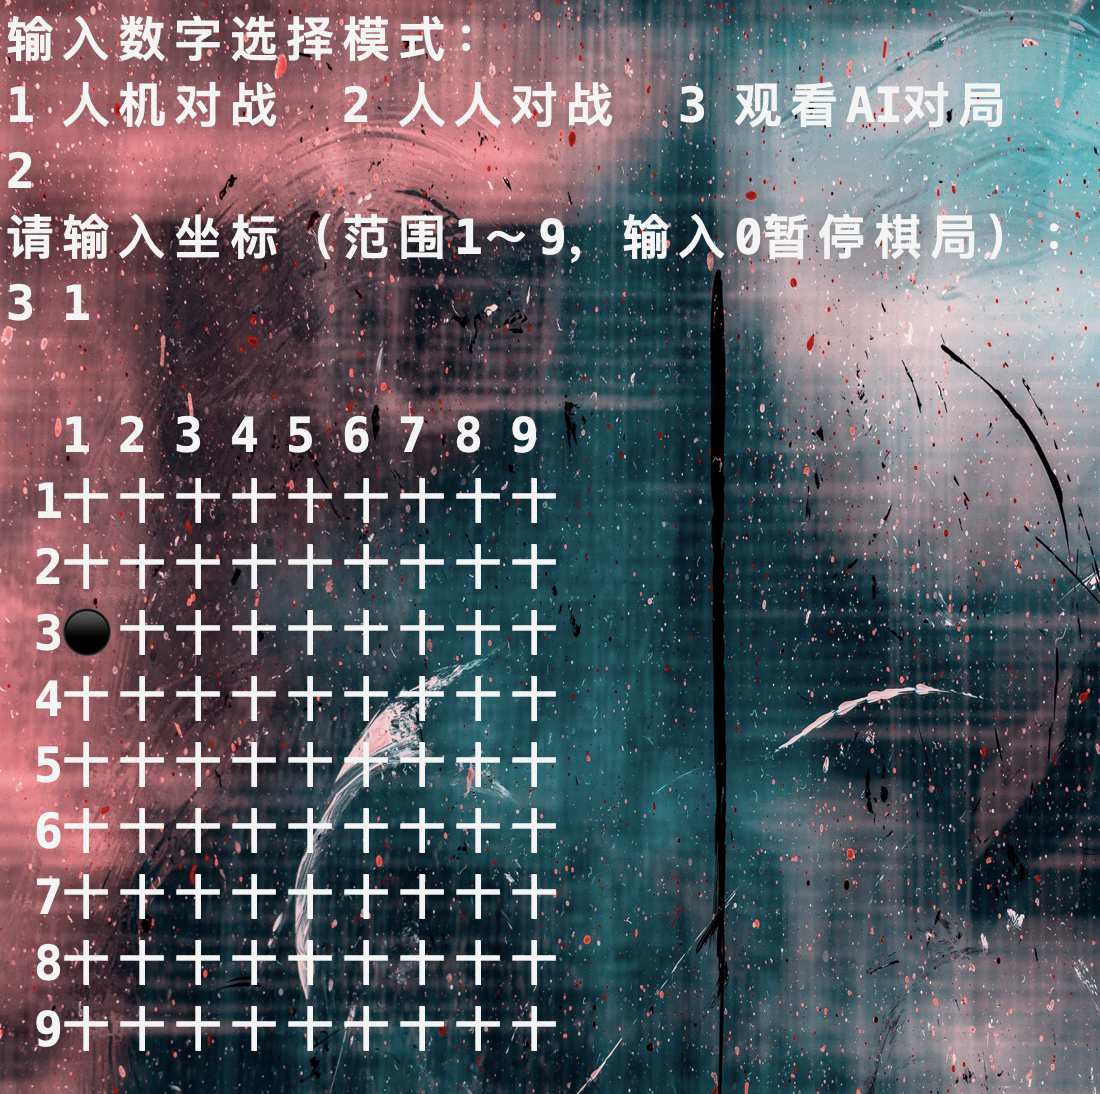
\includegraphics[width=0.4\textwidth]{fig7}
\caption{人人对战的终端交互界面}
\label{Fig5}
\end{figure}
\subsection{辅助功能}
\subsubsection{菜单界面}
在任意需要输入棋盘坐标的时刻,输入0即可呼出暂停菜单界面,如图\ref{Fig6}所示,可以选择悔棋、继续游戏、开始新游戏或结束棋局。
\begin{figure}[H]
\centering
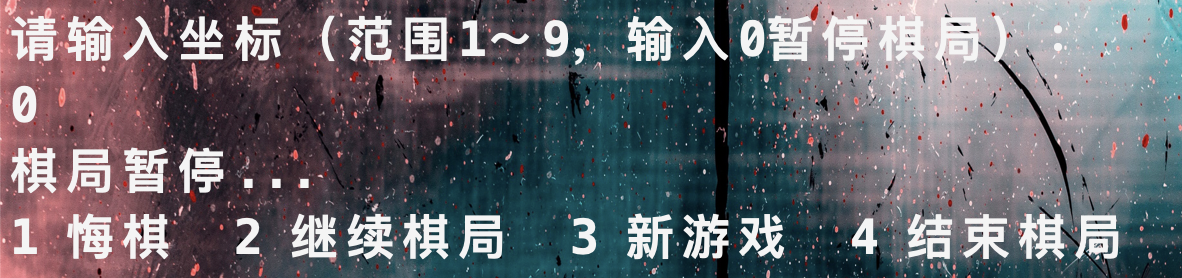
\includegraphics[width=0.4\textwidth]{fig8}
\caption{暂停菜单界面}
\label{Fig6}
\end{figure}
悔棋功能针对人机对战模式和人人对战模式略有不同,在人机对战时撤回两步棋,人人对战时撤回一步棋,悔棋后的棋计入新的存档,复盘时不会显示被撤回的棋。未加入刷新界面命令时,悔棋功能示意如图\ref{Fig7}所示。
\begin{figure}[H]
\centering
\subfigure[人机对战撤回两步]{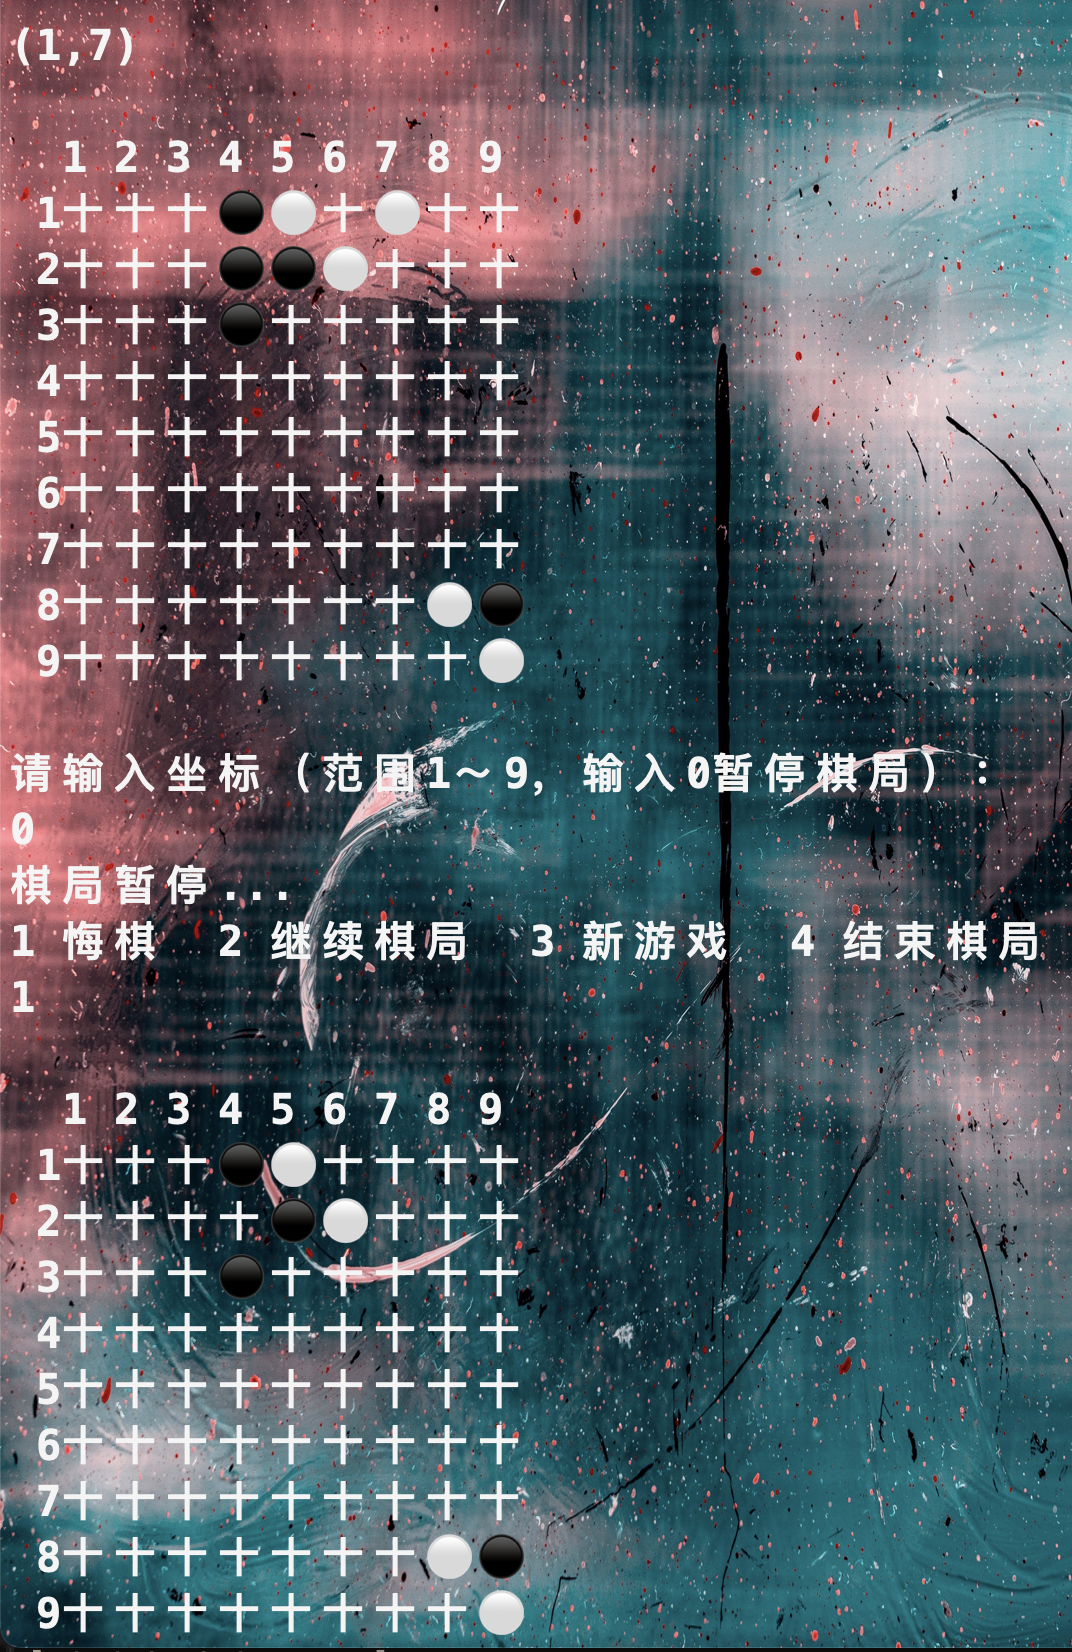
\includegraphics[height=6cm]{fig9}}
\subfigure[人人对战撤回一步]{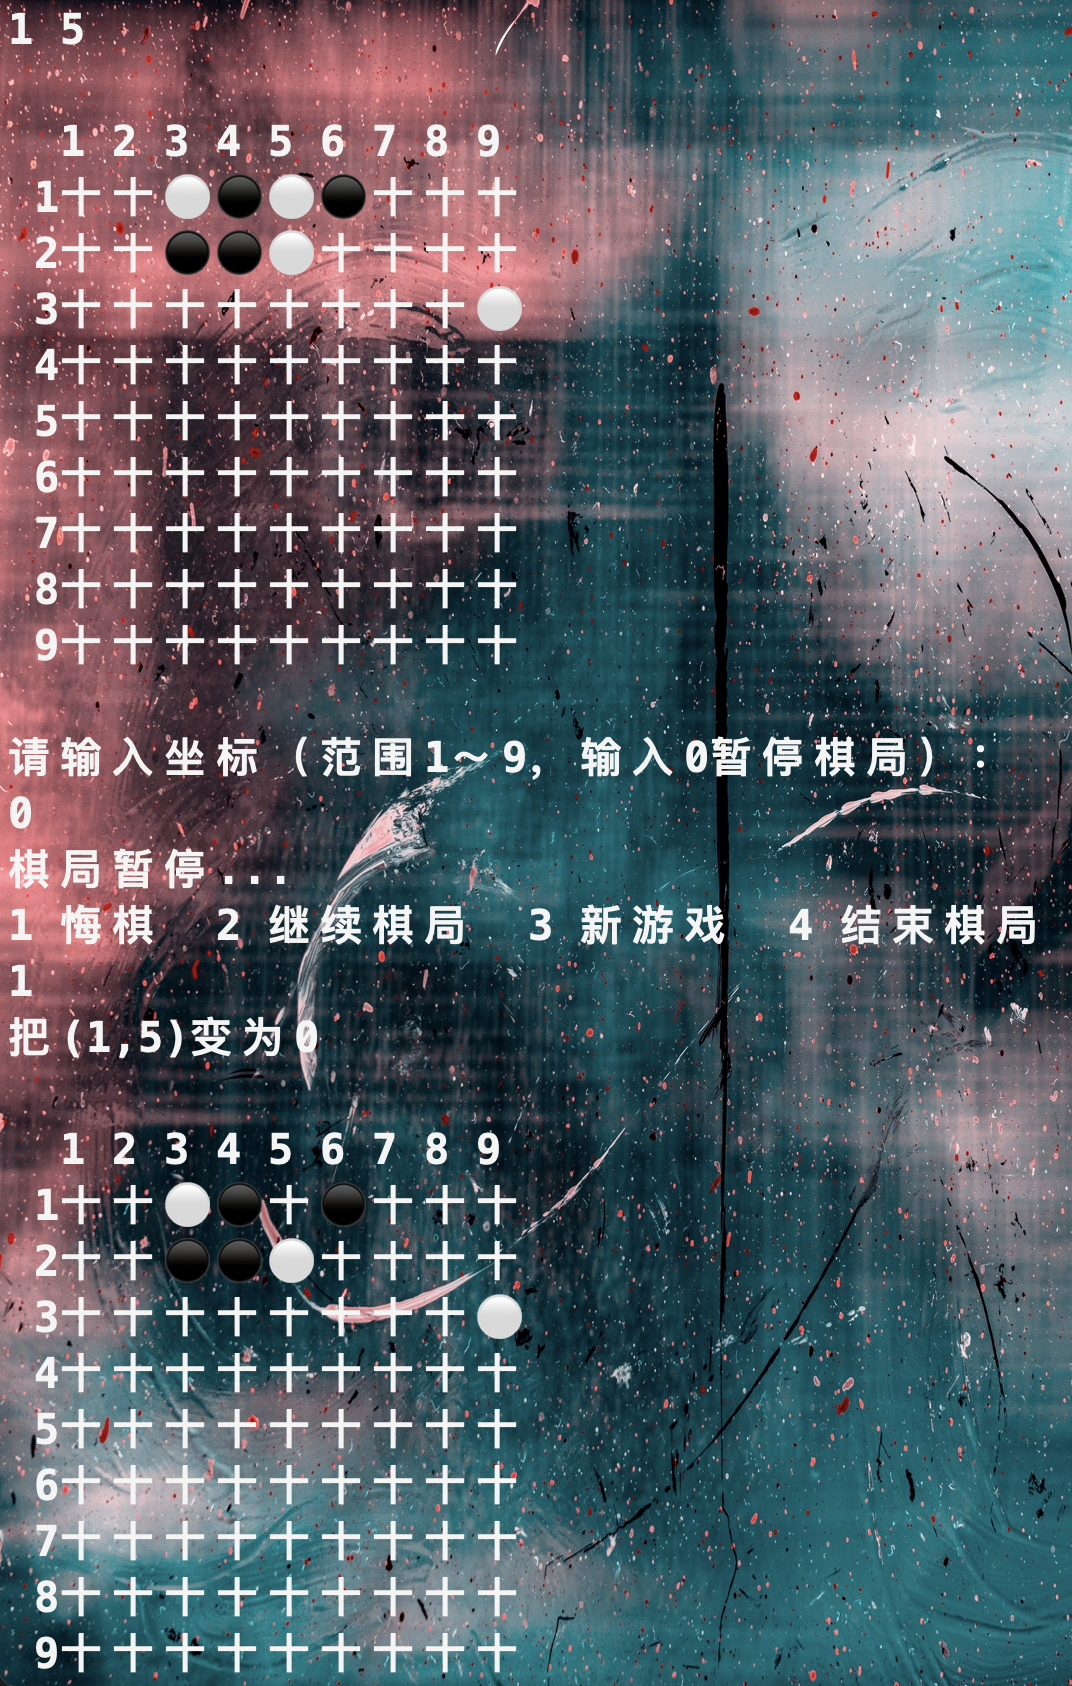
\includegraphics[height=6cm]{fig10}}
\caption{悔棋功能示意}
\label{Fig7}
\end{figure}
棋局因一方负而结束、或在暂停菜单中键入4结束棋局时,会呼出结束界面菜单(如图\ref{Fig8a}),可以选择复盘、新游戏或者退出程序。复盘功能通过在对战过程中自动存储的棋谱数据,从第一手棋开始,以每秒一步棋的速度匀速复盘直至最后一步棋(如图\ref{Fig8b}),便于玩家总结对弈经验。
\begin{figure}[H]
\centering
\subfigure[结束界面菜单]{\label{Fig8a}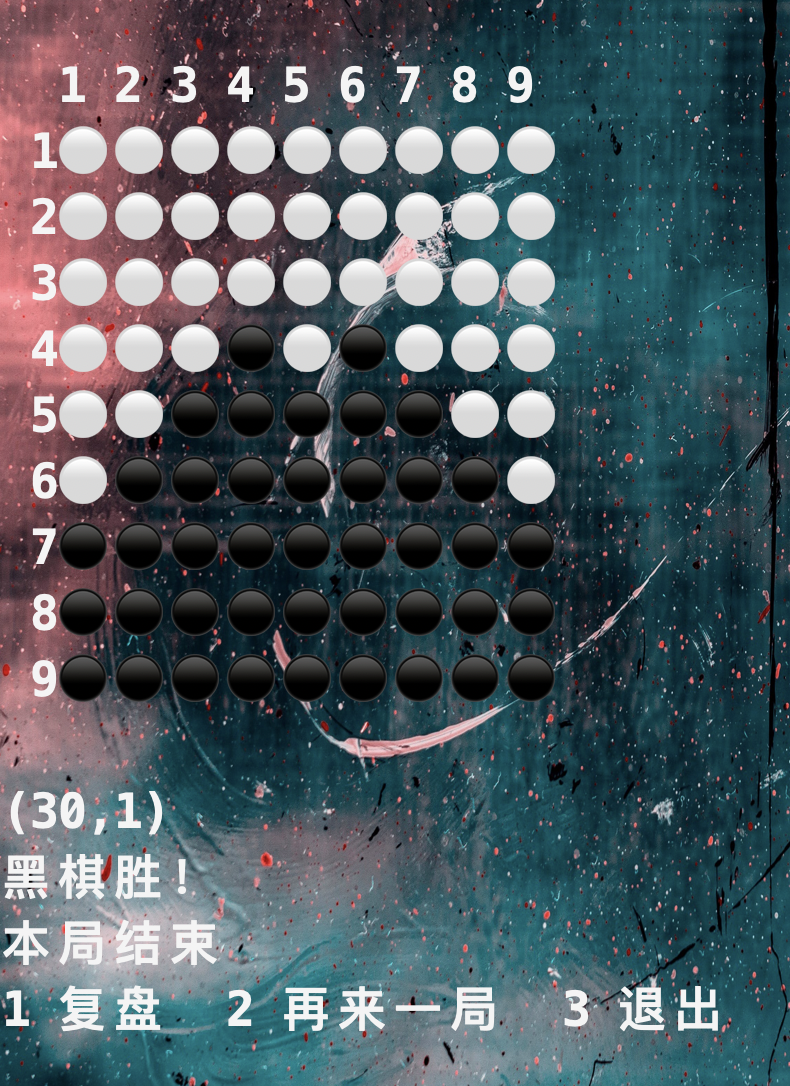
\includegraphics[height=7cm]{fig12}}
\subfigure[复盘输出流示意]{\label{Fig8b}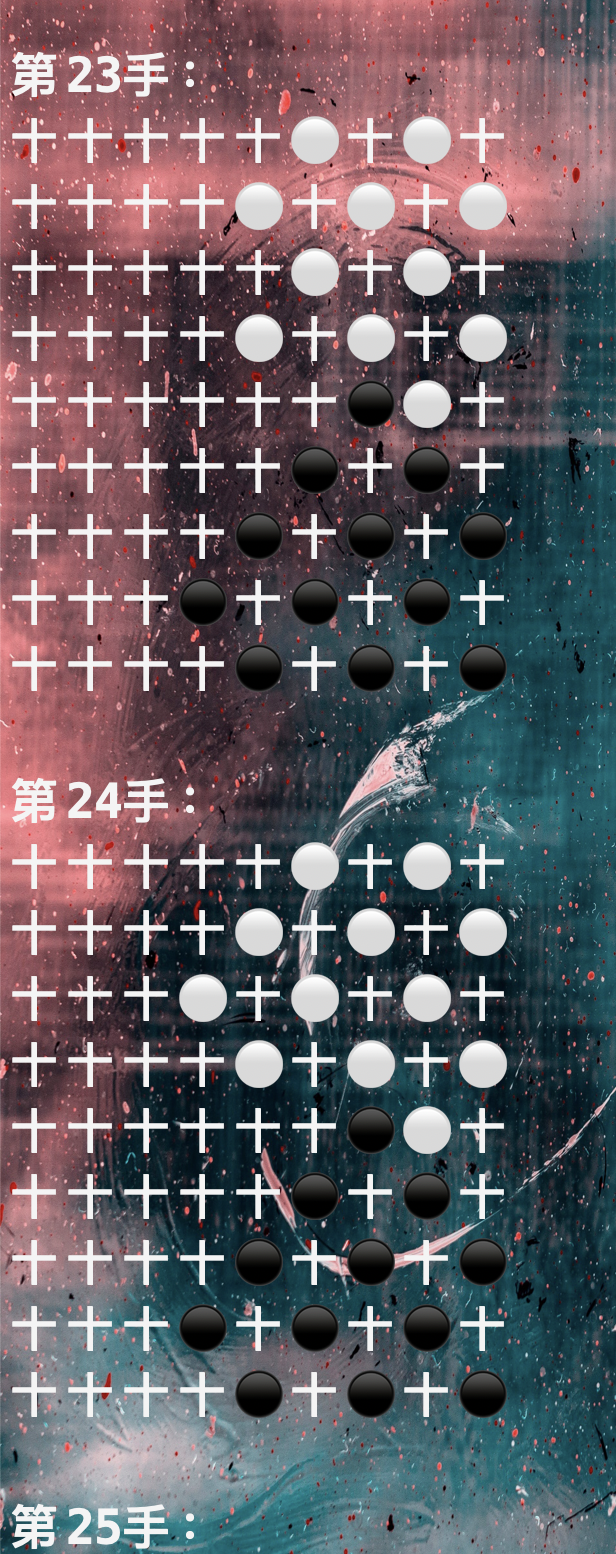
\includegraphics[height=7cm]{fig13}}
\caption{结束界面}
\label{Fig8}
\end{figure}
\subsubsection{智能提示}
基于对禁止点和死点的判断,游戏提供了智能提示功能。在对战时,若玩家输入的点范围越界,程序会自动提示“非法落子”,引导玩家重新输入。针对玩家容易出现误操作、输入死点或禁止点坐标的问题,程序提供了智能提示禁止点和死点的功能开关,开启开关后可以以此方式减少玩家失误的可能性。
\begin{figure}[H]
\centering
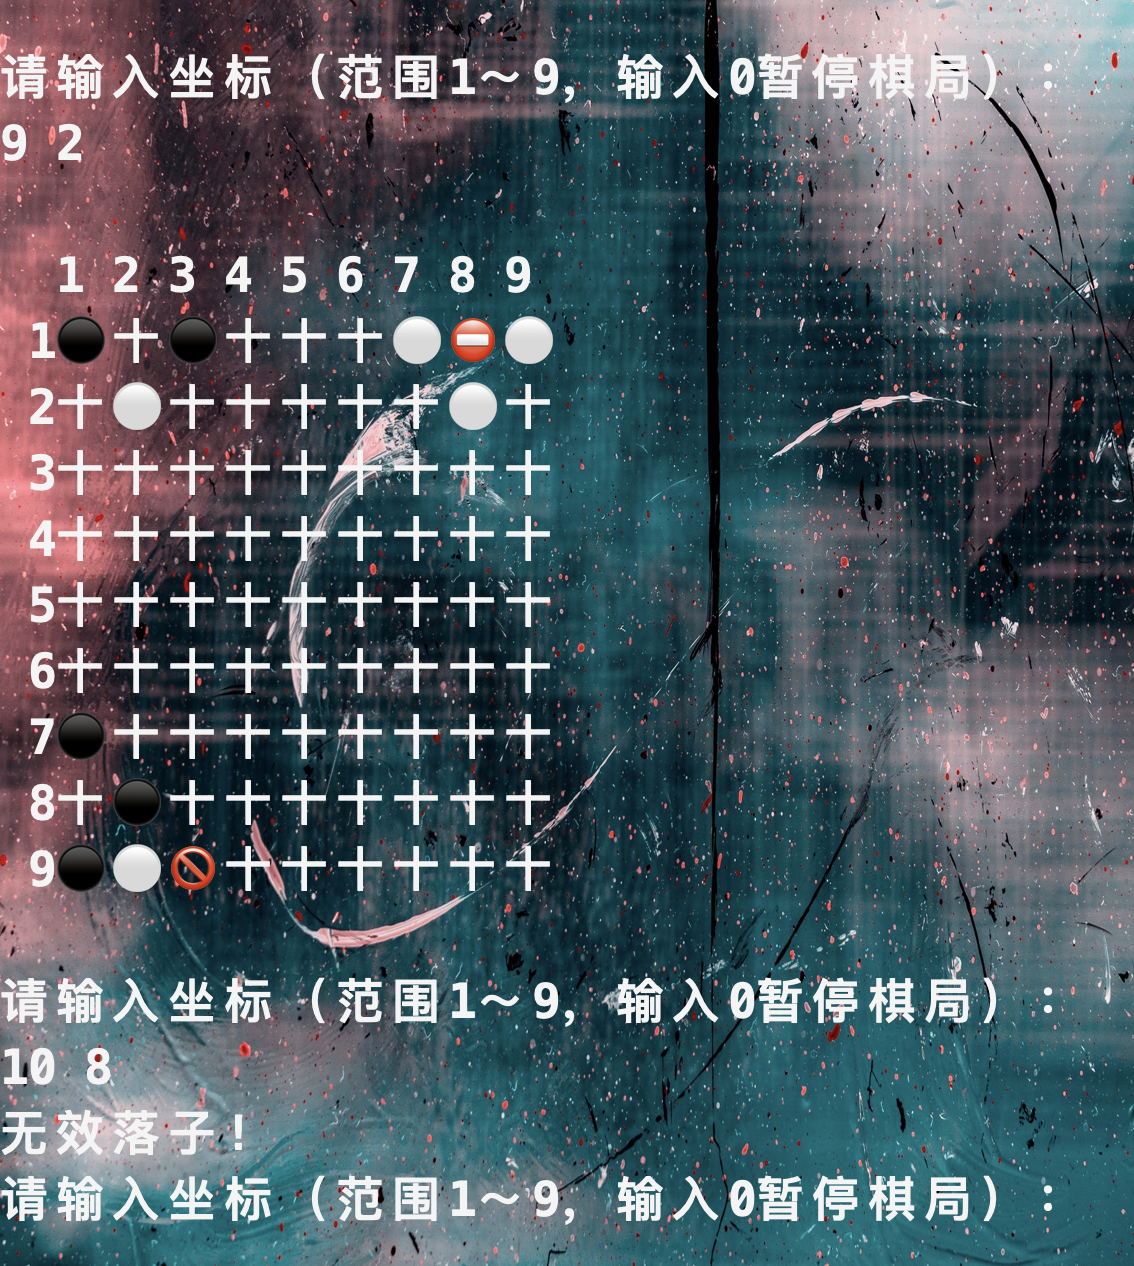
\includegraphics[width=0.4\textwidth]{fig14}
\caption{智能提示:无效落子与禁止点提示}
\label{Fig智能提示}
\end{figure}
\section{图形交互界面}
\subsection{界面展示}
利用EasyX上的图形库绘制开始界面、选择界面和棋盘界面。
\begin{figure}[H]
\centering  %图片全局居中
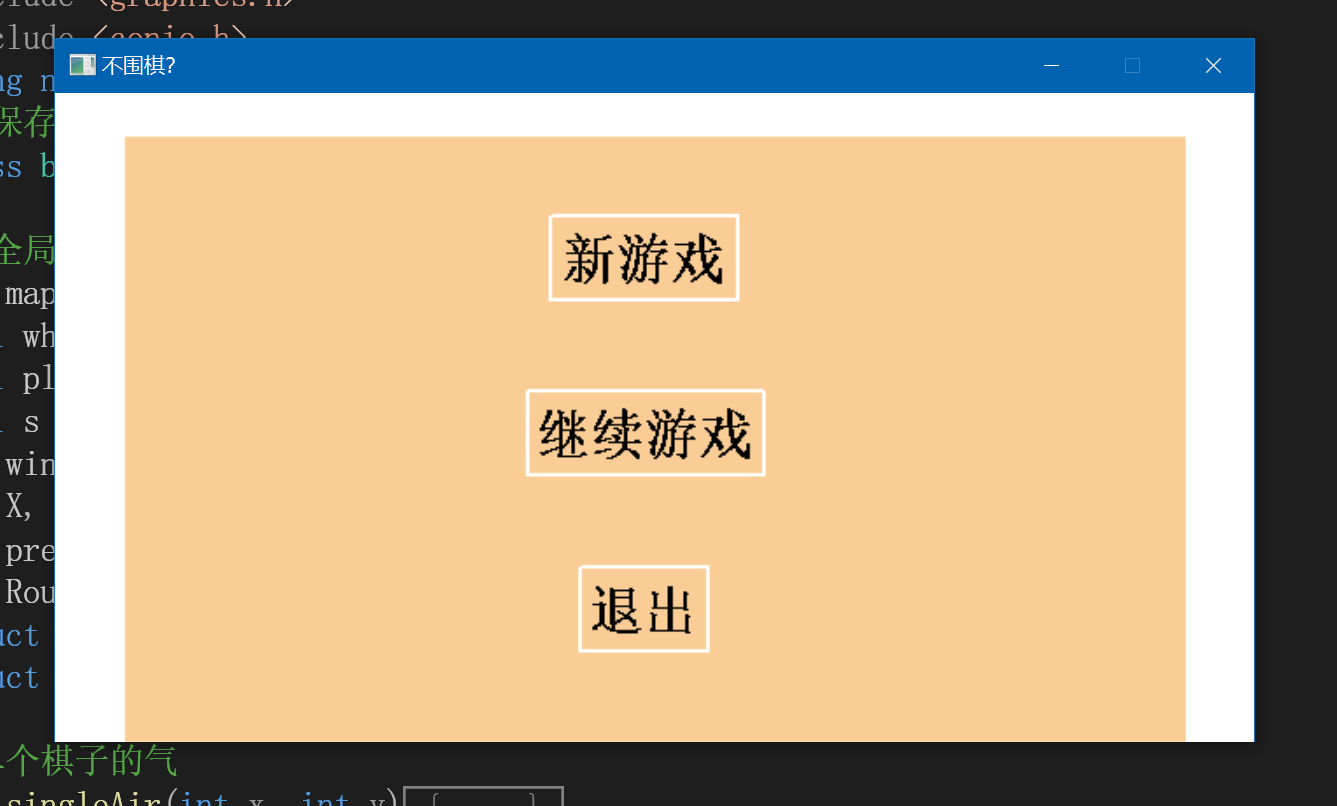
\includegraphics[width=0.47\textwidth]{start}
\caption{开始界面包括开始新游戏、继续游戏、退出的选择}
\label{Fig.main}
\end{figure}

\begin{figure}[H]
\centering  %图片全局居中
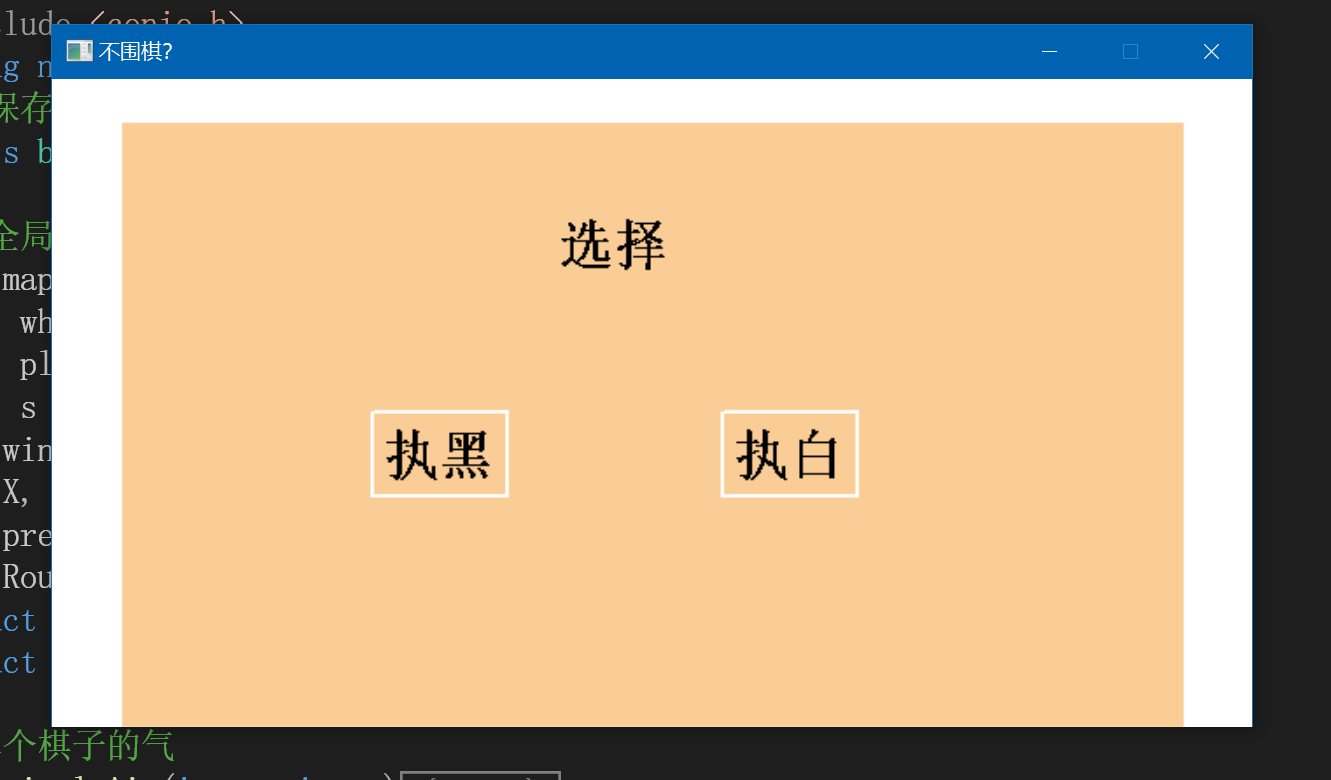
\includegraphics[width=0.47\textwidth]{choice}
\caption{在选择开始新游戏后,需要选择执黑或执白}
\label{Fig.main}
\end{figure}

\begin{figure}[H]
\centering  %图片全局居中
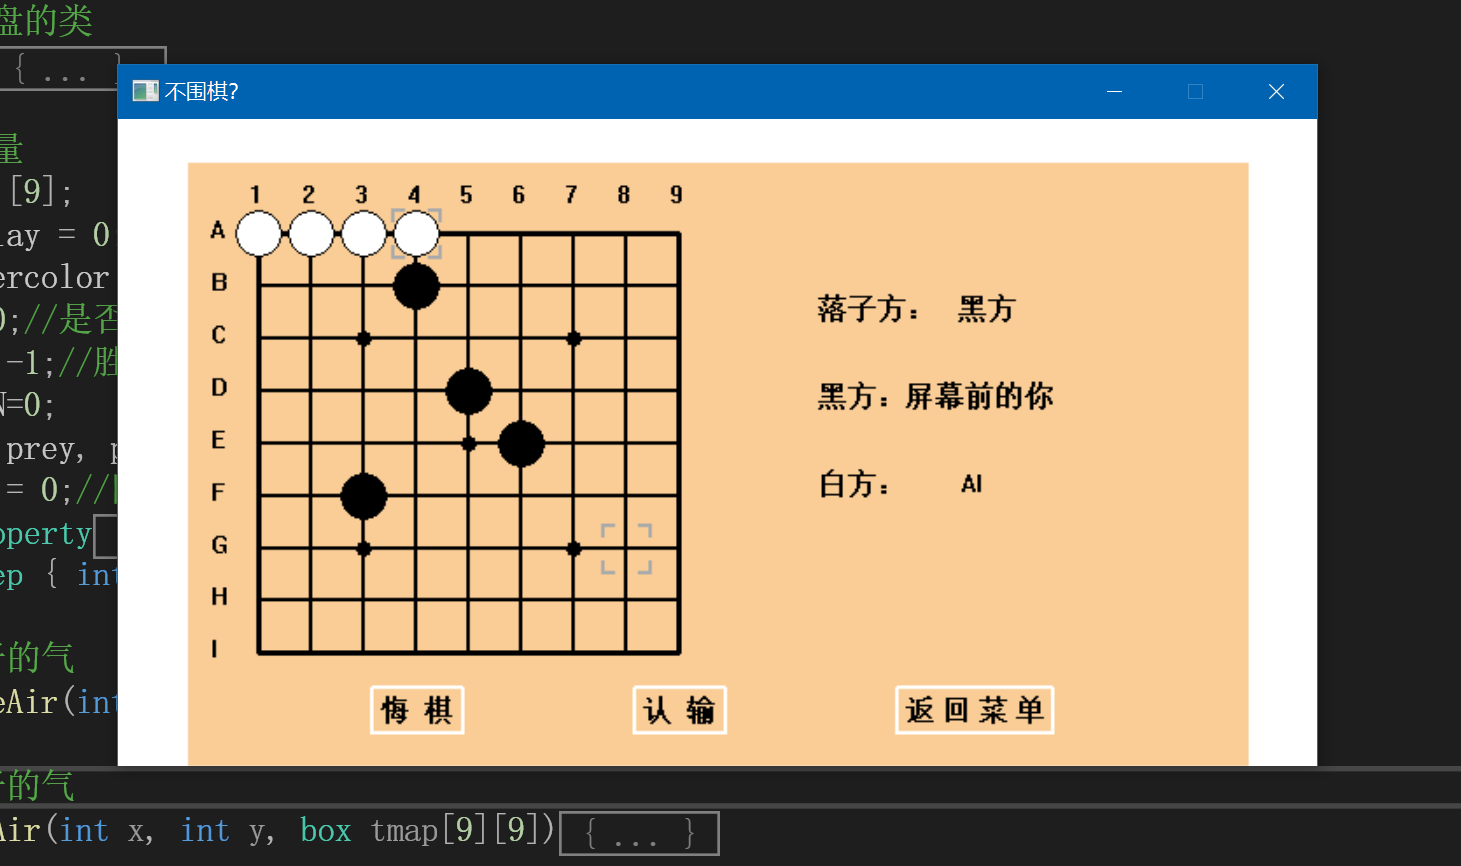
\includegraphics[width=0.47\textwidth]{map}
\caption{棋盘界面包括棋盘、黑白方、落子方的实时显示和悔棋、认输、返回菜单的选择。悔棋接受悔一步,返回菜单后也可以继续游戏。在落子时,光标移动到不同的位置会有选择框,左键单击便可以落子。
}
\label{Fig.main}
\end{figure}

\subsection{代码实现}

在棋盘的结构体数组中储存坐标、以数字代表的颜色、棋盘格线段模式、选择框和关于这些量的draw绘制函数。

\par

全局变量:棋盘的类、执子方、玩家颜色、是否退出、胜负判断、上回合的落子(用于悔棋)、回合数等。
\begin{lstlisting}[language=C++]
// 保存棋盘的类
class box
{
public:
	void draw();            // 绘制
public:
	int x = 0;              // x 坐标
	int y = 0;              // y 坐标
	int value = -1;         // 值(黑棋:1,白棋:0,空位:-1)
	int modle = 0;          // 模式
	bool isnew = false;     // 是否有选择框
	COLORREF color = WHITE; 
	// 棋盘背景色
};

// 全局变量
box map[9][9];      // 棋盘
bool whoplay = 0;      // 轮到谁下棋了
bool playercolor = 0;  // 玩家颜色
bool s = 0;//是否退出
int win = -1;//胜负
int X, Y,N=0;
int prex, prey, prexx, preyy;
//上一回合下的棋
int Round = 0;//回合数
struct property
{
	int val;
	int myEye;
	int commonEye;
	int myDeadPoint;
	int myTigerPoint;
	int eneEye;
	int eneDeadPoint;
	int eneTigerPoint;
};
struct step 
{ int x; int y; int chess; };
\end{lstlisting}
 
\begin{figure}[H]
\centering  %图片全局居中
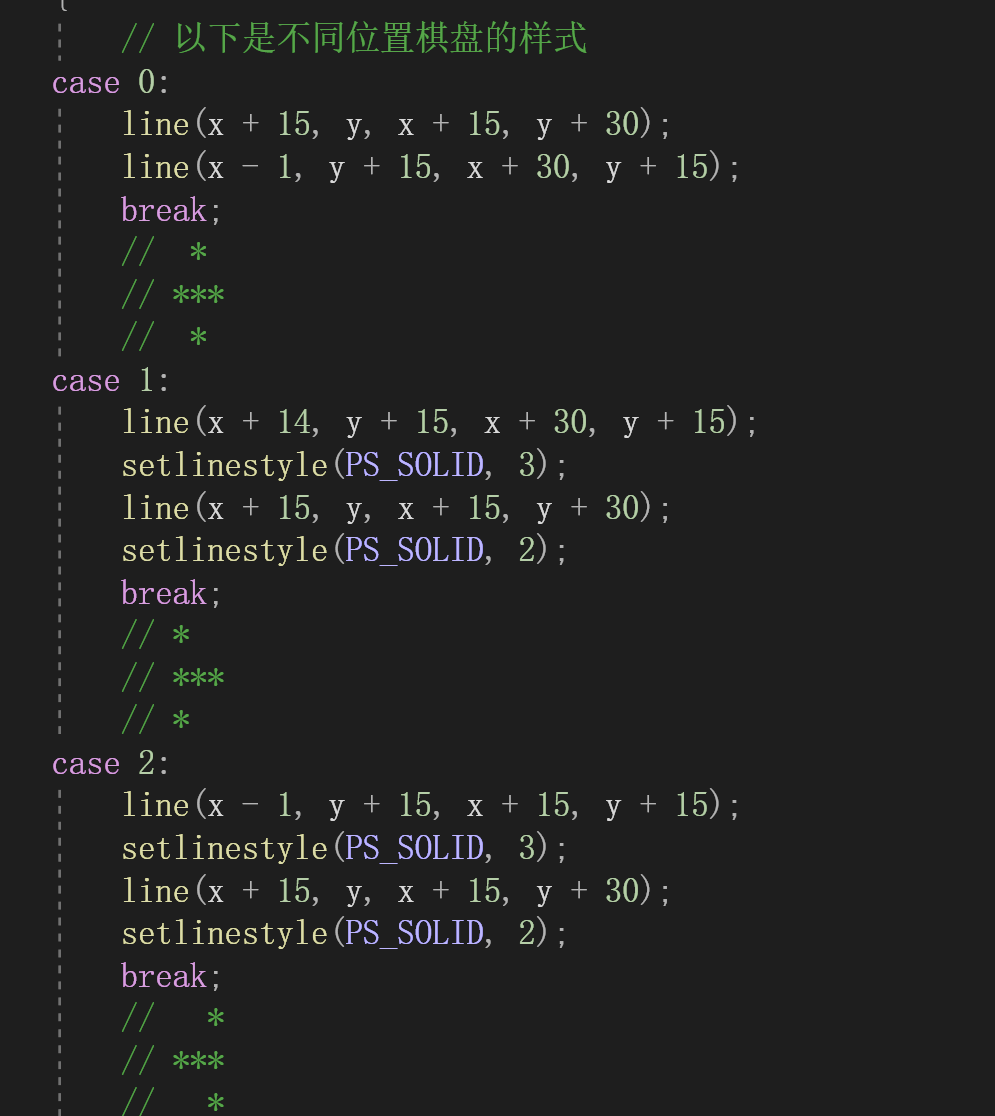
\includegraphics[width=0.4\textwidth]{chess}
\caption{不同样式的棋盘格线段}
\label{Fig.main}
\end{figure}

关于界面的函数,有输赢判断函数、开始界面函数、选择界面函数、结构体中的draw绘制函数和全局的draw绘制函数、初始化函数、游戏主函数。
\begin{figure}[H]
\centering  %图片全局居中
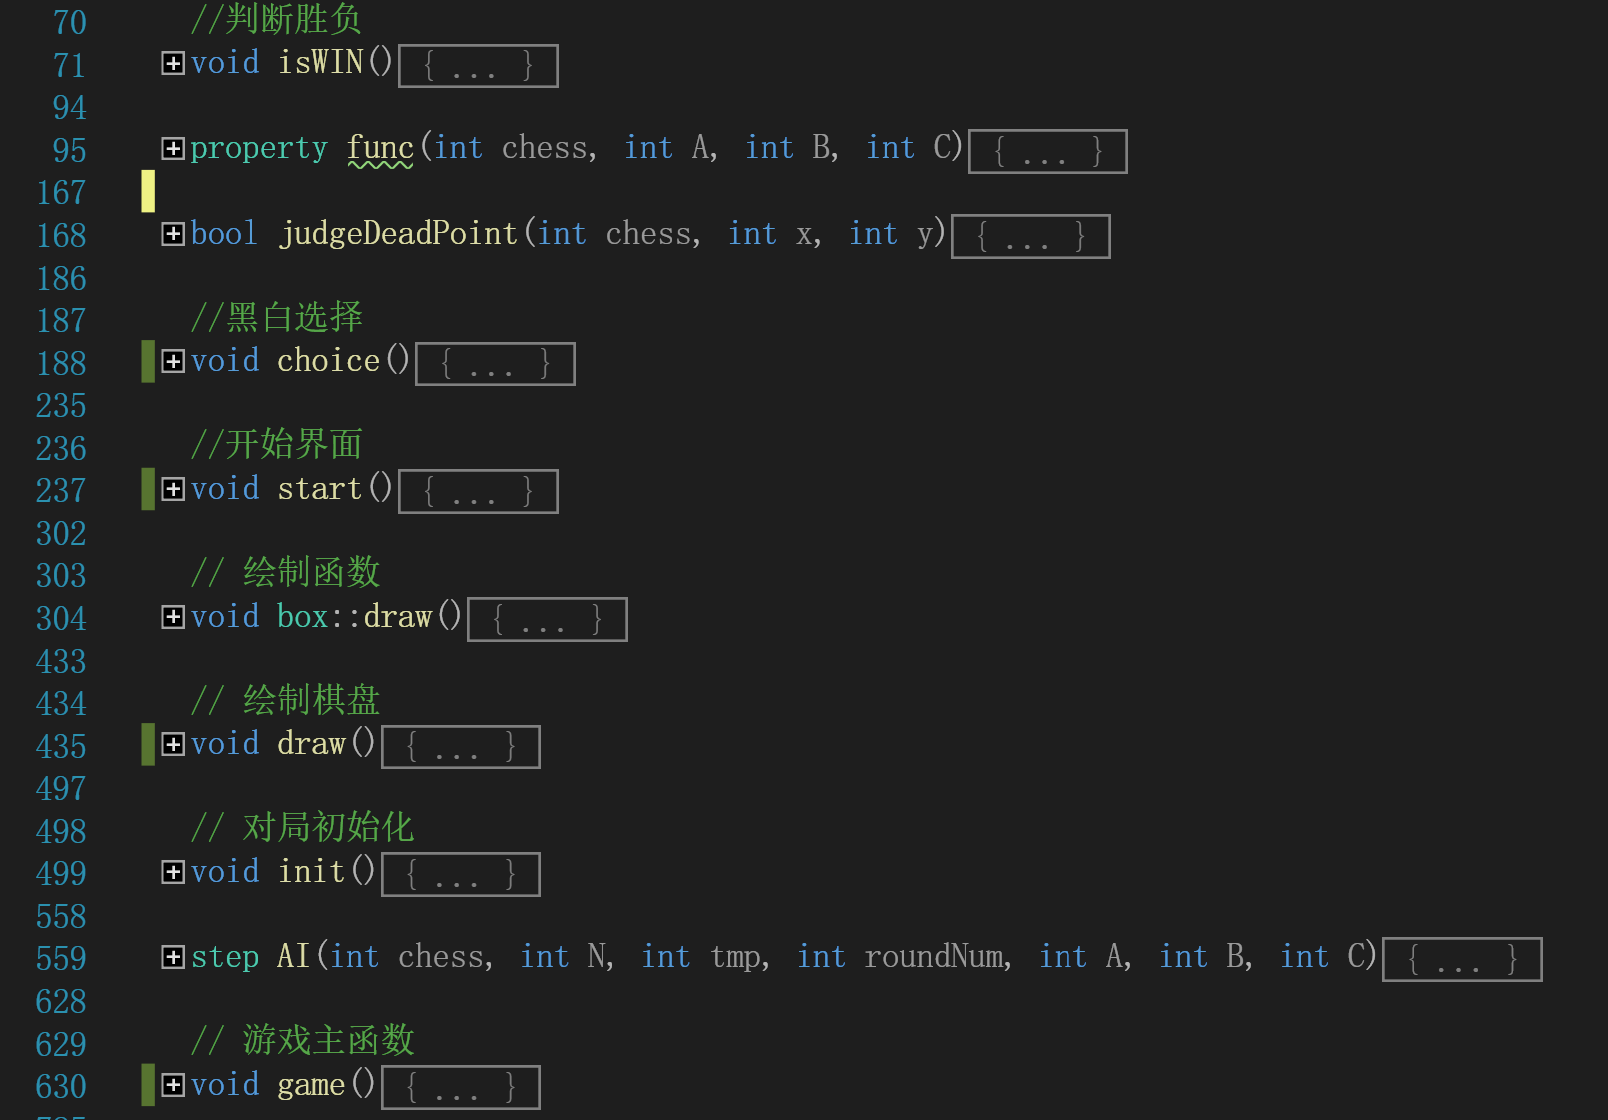
\includegraphics[width=0.4\textwidth]{func}
\caption{函数}
\label{Fig.main}
\end{figure}
 
main函数:初始化界面并转入game函数。
\begin{lstlisting}[language=C++]
int main()
{
  initgraph(685, 370); 
  // 初始化绘图环境
  setbkcolor(WHITE);
  cleardevice();
  setbkmode(TRANSPARENT); 
  // 设置透明文字输出背景
  init(); // 初始化
  game(); // 游戏开始	
}
\end{lstlisting}

在game函数中转入start函数,即开始界面,选择黑白子后,转入draw绘制棋盘界面,然后开始对战。
\begin{lstlisting}[language=C++]
void game(){
  bool isinit;// 上一个鼠标停的坐标
  int oldi = 0;
  int oldj = 0;
  // 绘制背景
  setfillcolor(RGB(250, 205, 150));
  solidrectangle(40, 25, 645, 630);
  start();
  if (s == 1) return;
  if (playercolor == 0){
  	isinit = 1;
	whoplay = 1;
  }
  else{
	isinit = 0;
 	whoplay = 1;
  }
  draw(); // 绘制
  while (1){
	NEXTPLAYER:
	......
	DRAW:
	......
 \end{lstlisting}
\par 
用MOUSEMSG进行鼠标交互,在一定的坐标内点击就可落子/悔棋/认输,落子后改变棋盘数组map的状态,然后goto DRAW,先判断输赢状态,再清屏进行绘制棋盘。如果输赢已定就输出输赢,并且在休息一段时间后返回主菜单。
\begin{lstlisting}[language=C++]
while (1)
{
  MOUSEMSG cho = GetMouseMsg();
  if (cho.y > 325 && cho.y < 351 
  && cho.x>145 && cho.x < 197)//悔棋
  {
  	if (cho.mkLButton)
  	{
    	map[prex][prey].value = -1;
	map[prexx][preyy].value = -1;
	goto DRAW;
	}
  }
  if (cho.y > 325 && cho.y < 351
   && cho.x>295 && cho.x < 347)//认输
  {......
 \end{lstlisting}
\newpage

 \part{总结}
 在这次不围棋大作业的制作过程中,我们体会到,一些看起来很简单的游戏背后,蕴含着很多很多内容——游戏算法、界面都需要我们不断地选择、调整、规划,在这个过程中我们遇到了很多困难,但在这些挑战中我们学习到了更多实用的代码操作,比如负极大值搜索、蒙特卡洛树、图形界面、鼠标交互等等,这使我们的编程能力有很大提升,也真正进入了一种开发程序的状态。总之,真是一段美妙的旅程!

 \begin{thebibliography}{99}  

\bibitem {ref 1}Q. Guo and Y. Chen, "Artificial Intelligence Algorithm for the Game of NoGo based on Value Evaluation," 2018 International Conference on Information Systems and Computer Aided Education (ICISCAE), Changchun, China, 2018, pp. 467-470, doi: 10.1109/ICISCAE.2018.8666845.
\bibitem  {ref 2}不围棋, 计算概论大作业, 2020.11.7.

\end{thebibliography} 
% ·-·-·-·-·-·-·-·-·-·-· [落笔成文] ·-·-·-·-·-·-·-·-·-·-· %
\end{document}